\section{A periodic loop calculation at finite circumference}\label{L:part1}

Set
\[
 q=e^{\pi i/4},\qquad k=2+\sqrt2,\quad X=k^{-1/2},
 \quad \kappa=k-1=1+\sqrt2 .
\]
When half-powers of \(q\) occur we use this particular angle. Consider an infinite combinatorial cylinder of rhombi (a square grid suffices topologically), \(N\) per horizontal row. There are ports (side midpoints) \(L,B,R,T\) (left, bottom, right, top) on each cell in that cyclic order, common to neighboring cells. A diagram in the cell is a noncrossing matching of a subset of these ports. In gluing diagrams the two occupations of each common port must agree; matchings then join across it, weights multiplying. Use configurations with finite support. For a ratio \(s=z_j/t=e^{3ig/4}\) in column \(j\), put \(\eta=3g/8\) (so \(e^{i\eta}=z_j^{1/2}/t^{1/2}\)), \(D=\sin(5\pi/4+\eta)\sin(5\pi/8-\eta)\). Weights are 1 for vacant,
\[
 u=\sin(5\pi/4)\sin(5\pi/8+\eta)/D,\quad
 U=\sin(5\pi/4)\sin\eta/D,\quad
 v=-\sin(5\pi/8+\eta)\sin\eta/D
\]
for a single arc (\(LT\) or \(BR\); \(LB\) or \(TR\); opposite sides respectively), and
\[
 w=\sin(5\pi/8+\eta)\sin(5\pi/4-\eta)/D,\qquad
 W=-\sin(15\pi/8+\eta)\sin\eta/D
\]
for \(LT,BR\) and \(LB,TR\), respectively (the Yang--Baxter rhombus weights; the identities needed here are checked below). At \(s=q\) (the indicated half-power branch) this is the honeycomb SAW weight: split the rhombus into unit equilateral triangles, one with sides \(L,T\), one with \(B,R\), each supporting a single arc between two distinct side midpoints via the center with weight \(X\) (or vacant with weight 1). Thus the walk goes between centers, with weight \(X\) per visited vertex. At \(s=q^2\) the reflected picture holds. The regular cylinder quotient in either case is by translation along a horizontal row of triangle sides. \cite{GlazmanManolescu2017}

Mark the auxiliary port \(L\) of column 1 (the seam), in one row. Consider configurations consisting of precisely one loop, with weights given by the indicated cells, homogeneous up and down the cylinder. Let \(E_+(Z;t)\) denote their mass when required to contain the mark. Here \(Z=(z_1,\ldots,z_N)\). Let \(J(Z;t)\) denote instead the mass of single winding loops modulo translations by whole rows (no mark condition, and quotient by vertical/row translations only, NOT cyclic shifts of columns). Initially these sums can be taken at the regular honeycomb point and in a neighborhood; elsewhere we will use rational continuation.

Use the following notation:
\[
 \begin{aligned}
 h(x,y)&=x^2+y^2+\sqrt2 xy,\qquad K(x,y)=(x^2+y^2)h(x,y),\\
 d(x,t)&=(x-q^5t)(x-q^6t),\quad
 F(Z)=\prod_{i<j} h(z_i,z_j)/(z_i-z_j),\\
 Q(Z)&=F(Z)\operatorname{Pf}_{\rm ext}[(x^2-y^2)/h(x,y)]_{x,y\in Z},\\
 M(x,y)&=kxy/h(x,y),\qquad R(Z)=F(Z)^2\det M(Z,Z),\\
 Y(Z)&=\kappa^N Q(Z)^2/R(Z),\\
 p_Z^\pm(s)&=s^{\pm1}-M(s,Z) M(Z,Z)^{-1}(z^{\pm1})_{z\in Z}.
 \end{aligned}
\]
Augment the Pfaffian by a last column 1 (with the skew row) in odd size only. Determinantal quotients etc. mean rational functions, so limits or continuation from distinct parameters are understood.

For the color sum choose constants $b_0=k$, $b_+b_-=k/2$ and
$b_++b_-+k=r$, and define
\[
\begin{aligned}
 S(u)&=(u+1)^2/[(u-q)(u-q^{-1})],\\
 P_{++}&=P_{--}=1,\qquad P_{00}(u)=S(u),\\
 P_{+0}(u)&=P_{0-}(u)=S(u/q),\\
 P_{+-}(u)&=S(u/q)S(u/q^2),\qquad P_{ba}(u)=P_{ab}(1/u).
\end{aligned}
\]
Set
\begin{equation}\label{L:eq:color-definition}
 O_Z(r)=\frac{\prod_{i<j}K(z_i,z_j)}{R(Z)^2}
 \sum_{\alpha\in\{+,0,-\}^N}
 \prod_i b_{\alpha_i}\prod_{i<j}P_{\alpha_i\alpha_j}(z_j/z_i).
\end{equation}
All quotients are interpreted as rational functions and then continued to
coincident parameters.

\begin{proposition}[Finite cylinder identities]\label{L:prop:periodic}
For the above periodic model, the marked-loop mass, winding-loop mass
modulo row translations, and color sum satisfy
\begin{align}
 E_+(Z;t)&=1+\kappa\left(\frac{Q(Z,t)Q(Z,q^3t)}
 {Q(Z)^2\prod_{z\in Z}d(z,t)}-1\right),\label{L:eq:one-port}\\
 Y(Z)J(Z;t)&=\frac{(-1)^{N+1}}{\sqrt2}
 [p_Z^+(t)p_Z^-(q^3t)+p_Z^-(t)p_Z^+(q^3t)],\label{L:eq:winding}\\
 O_Z(1)&=1,\qquad O_Z(\kappa)=Y(Z),\qquad
 O_Z(\kappa^2)=Y(Z)^2.\label{L:eq:color-values}
\end{align}
These identities hold initially at physical parameters and their
convergence neighborhoods, and elsewhere by rational continuation.
Replacing $q$ by $q^{-1}$ in the color factors has the same effect as
exchanging $+$ and $-$, including $b_+,b_-$.
\end{proposition}

The relation between parafermionic cancellation, rhombic geometry and
integrable loop weights was developed by Ikhlef and Cardy
\cite{IkhlefCardy2009}. Glazman's treatment gives the corresponding
weighted-walk criticality and corrected general loop-weight formulas
\cite[Theorems~1.1--1.2 and Section~5]{Glazman2015}. We verify the particular normalizations and
all diagram identities used here.

We prove Proposition~\ref{L:prop:periodic} in three steps: construct the actual convergent vacua, determine their polynomial numerators, and glue them with the required mark or twist. The boundary estimate needed for the first step is proved next. At a horizontal slice the lower vacuum \(V^\sigma\) has one component (weighted sum) for each pairing of a subset of the \(N\) ports, noncrossing on the disk. It accumulates diagrams closed below the slice except for precisely these ends (no closed loops), with an extra factor \(\sigma\) for every occupied horizontal seam-crossing port, \(\sigma=\pm1\). We forget homotopy beyond this sign. Noncrossing is necessary also on the half-cylinder (cap off below a finite diagram). In particular \(V^\sigma_\emptyset=1\). Row addition \(T_\sigma(Z;t)\) acts linearly, killing \emph{any} resulting cycle, and including the extra seam factor also in the added row. That is, each column of this finite matrix attaches one row in all possible ways just above the specified input pairing; what is needed from the input is only which ends are joined, since cycles of either topology are discarded. The empty input vector refers to the unit coordinate for the all-vacant state.

Here are convergence/uniqueness details for this construction. A single arc in such a half-cylinder at the honeycomb point lifts to a half-plane SAW between boundary mid-edges (touching that boundary only at its two ends). The total \(X\)-mass of such SAWs from a fixed port is finite, even summed over all other boundary ports. To see this, exhaust by convex polygons made of equilateral triangles on that side with the source in the interior of a bottom side. For a midpoint \(s\) use the sum \(f(s)\) of walks terminating there in the polygon, weighted by \(X^{\#\text{vertices}}\exp(-5i\,{\rm turn}/8)\) ('turn' is total signed turn of travel), starting at the boundary source in the inward direction and not touching the boundary intermediately; include the empty walk with weight 1. At a triangle center \(v_0\),
\(\sum_{s\sim v_0}(s-v_0)f(s)=0\).
Indeed contributions for a walk approaching an unvisited \(v_0\), and its two extensions to exit midpoints there (turns \(\pm\pi/3\)), cancel by \(1+2X\cos(7\pi/8)=0\). A walk stopping while approaching \(v_0\) which was already visited pairs with the reversal of the detour since that visit (thus using the other exit from \(v_0\)); the incoming leg at the earlier visit is on the outside of the simple polygon closed by the detour (it is reached from the boundary without crossings). The added turns starting from this leg are \(4\pi/3,-4\pi/3\) (the positively oriented polygon contributes \(2\pi-\pi/3\) without its closure bend, and the entry bend is \(-\pi/3\); likewise for negative orientation); for terminal rays from the center at angles 0 and \(-2\pi/3\) respectively the coefficients cancel by \(e^{-5i\pi/6}+e^{-2i\pi/3+5i\pi/6}=0\), and rotations/reflection give the other cases. Thus summing over centers leaves only boundary terms; divided by the inward source direction (times the common half-edge length), this gives that the sum of \(X^{\#\text{vertices}}\exp(3i\,{\rm turn}/8)\) over nonempty exits is 1. Closing a nonempty simple arc counterclockwise along the convex boundary shows the turn from inward to outward normal has absolute value at most \(\pi\) (total \(2\pi\), with two extra \(\pi/2\) corners and boundary contribution between 0 and \(2\pi\)). Taking real parts gives total exit mass at most \(1/\cos(3\pi/8)\). This proves the bound by exhaustion. This is the boundary parafermionic cancellation at the honeycomb critical activity \cite{DuminilCopinSmirnov2012}. The local cancellation and the boundary flux equality need no convexity provided the detour polygon cannot enclose the source (as for an outer boundary source with all detour edges interior); convexity here is for uniform positivity.

Dropping mutual avoidance now bounds all components of \(V^+\) (the number of ends at most \(N\)). They are limits of \(T_+^m\) on the empty input. At \(s=q\), each pairing is accessible with positive weight from that input: working \emph{down} from the slice, join adjacent paired ends (after previous joins) in a fresh row with corners and horizontal propagation, propagating all other ends vertically, iterating. This uses noncrossing and single arcs only. Since the empty row-output functional only sees the empty input, convergence of the monotone series for every state and this accessibility imply summability of powers of the nonempty block, so its spectral radius is \(<1\) (the same reflected argument at \(s=q^2\)). Absolute domination handles the twist and a small complex neighborhood by continuity, including convergence of marked sums via gluing two half-cylinders. Thus \(V\) there is characterized by \(T V=V,\ V_\emptyset=1\).

\begin{remark}[Critical activity and unfolding]
The preceding boundary bound proves vacuum convergence. We also recall how it identifies the critical activity, to keep the normalization self-contained. For completeness \(X\) here really is the inverse connective constant. First, plane vertex bridges between two distinct horizontal heights (heights of vertices, with all other vertices between, ties allowed) have bounded total \(X^{\#\text{edges}}\)-weight uniformly for fixed starting vertex and span. Extend their extrema outwards to boundary mid-edges on the nearest parallel lines of triangle sides on either side (at most one extra vertex at each end before that midpoint, always strictly outwards so unused). This gives simple crossings of that strip with only bounded multiplicity and weight factor, and the same convex exhaustion flux bound applies. Use the classical unfolding idea \cite{HammersleyWelsh1962,MadrasSlade1993}: decompose any \(n\)-step vertex walk, splitting in both directions from a lowest point, into such bridges by going to the \emph{last} subsequent extreme point in the given direction, then reversing (up/down) and repeating. Nonconstant remaining paths have a nonzero span (adjacent vertices have different heights). Within each half the successive spans decrease strictly except possibly the second equaling the first. In discrete height units their sum is \(O(n)\), so there are \(O(\sqrt n)\) pieces and at most \(\exp(O(\sqrt n\log n))\) choices of span lists. For a walk from a fixed origin the lowest point is in a set of \(O(n^2)\) possibilities. Multiplying the bridge bounds then gives subexponential total \(X^n\)-weight.

Conversely, suppose the plane walk series at \(X\) were finite. In an infinite strip between horizontal triangle-side lines at \(m\) rows' separation, start at a boundary mid-edge, and let \(A_m,B_m\) be the \(X\)-masses of nonempty arcs (mid-edge weights) returning to that side or reaching the other side before any other boundary contact. The same identity on exhaustion, now dropping remote exit terms by the assumed summability, gives \(1=\cos(3\pi/8)A_m+B_m\) from turns \(\pm\pi\) and 0. Moreover \(0\le A_{m+1}-A_m\le c B_{m+1}^2\) with constant \(c\): each new arc enters the outermost row; split at an extremal (farthest) vertex there and extend it on each half to the same far boundary port using at most one extra vertex strictly farther out. This gives two bridges, the first from the fixed source, the next back from its tip, with bounded multiplicity and weight comparison. Boundary ports on either side give the same crossing bound by symmetry. Hence \(1/B_m\) increases by at most a constant per row, so \(\sum_m B_m\) diverges, contradicting summability since their terminal heights differ. These plane mid-edge versus vertex conventions differ by only bounded endpoint choices and constant weight factors. Thus the plane series already diverges at \(X\), while it converges strictly below \(X\) by the subexponential bound, proving the radius assertion. The plane counts by edge length from a fixed vertex are submultiplicative by dropping mutual avoidance of consecutive blocks and using vertex transitivity, so this radius also gives the growth limit (divide lengths into blocks of any fixed size and a bounded remainder).

\end{remark}

\subsection{Diagram identities}\label{L:step1}

Interpret the same cell as a two-line swap \(B(s)\), with \(L,B,R,T\) interpreted respectively as old first, old second, new second, new first ports ('first' on the left in an ordered sequence of lines). Its argument when exchanging rapidities is right divided by left (before the swap). Thus a row is an auxiliary line initially on the left successively exchanged through all columns, then closed round to itself. In the diagram calculus compose linearly by gluing, dropping any term with an occupation mismatch or with a closed cycle formed; these matching identities can then be applied also to the vacuum pairing states. The triangle map \(P\) replaces one line by two neighboring lines and has the empty diagram and the three single arcs of weight \(X\). The cap map \(C\) replaces no lines by two with either no arc or a cup of weight 1. A transposed map reverses inputs and outputs. At adjacent rapidities \(q m,m/q\) (in that order) the lower vacuum will use \(P\) on a line of rapidity \(m\). At \(q^3 l,l\) it will use \(C\). Indeed \(B(1)=1,\ B(q^2)=P P^t,\ B(q^3)=CC^t\). One can pass these maps through a line of arbitrary rapidity (sliding the triangle/cap), going between two swaps and one/zero on the fused/removed side. Also swaps satisfy inversion and the ordinary braid relation with rapidity ratios.

Figure~\ref{L:fig:local-states} records the local states and port conventions.
\begin{figure}[tbp]
\centering
\begingroup
\newcommand{\FiniteSquare}[3]{%
  \begin{scope}[shift={(#1,#2)}]
    \draw[finite boundary] (-.35,-.35) rectangle (.35,.35);
    #3
    \foreach \p in {(-.35,0),(0,-.35),(.35,0),(0,.35)}
      \fill[black!45] \p circle (1pt);
  \end{scope}}
\newcommand{\FiniteTriangle}[3]{%
  \begin{scope}[shift={(#1,#2)}]
    \draw[finite boundary] (-.48,-.33)--(.48,-.33)--(0,.51)--cycle;
    #3
    \foreach \p in {(0,-.33),(-.24,.09),(.24,.09)}
      \fill[black!45] \p circle (1pt);
  \end{scope}}
\newcommand{\FiniteCap}[3]{%
  \begin{scope}[shift={(#1,#2)}]
    \draw[finite boundary] (-.48,.22)--(-.48,-.35)--(.48,-.35)--(.48,.22);
    #3
    \foreach \p in {(-.30,.22),(.30,.22)}
      \fill[black!45] \p circle (1pt);
  \end{scope}}
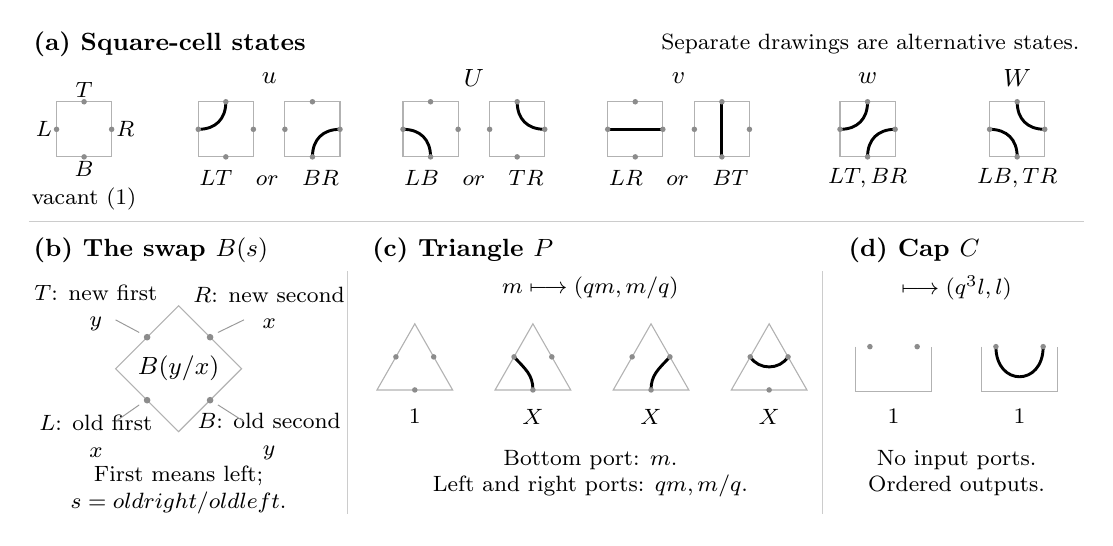
\begin{tikzpicture}[
  x=1cm,y=1cm,
  font=\small,
  finite boundary/.style={draw=black!30,line width=.4pt},
  finite arc/.style={draw=black,line width=1.05pt,line cap=round},
  every node/.style={inner sep=1.5pt},
  finite label/.style={font=\footnotesize},
  finite heading/.style={anchor=west,font=\small\bfseries}
]
  \node[finite heading] at (0,0) {(a) Square-cell states};
  \node[anchor=east,font=\footnotesize] at (13.4,0)
    {Separate drawings are alternative states.};

  \FiniteSquare{.70}{-1.08}{}
  \node[finite label,left]  at (.35,-1.08) {$L$};
  \node[finite label,below] at (.70,-1.43) {$B$};
  \node[finite label,right] at (1.05,-1.08) {$R$};
  \node[finite label,above] at (.70,-.73) {$T$};
  \node[finite label] at (.70,-1.96) {vacant ($1$)};

  \node at (3.05,-.43) {$u$};
  \FiniteSquare{2.50}{-1.08}{%
    \draw[finite arc] (-.35,0) .. controls (-.13,0) and (0,.13) .. (0,.35);}
  \FiniteSquare{3.60}{-1.08}{%
    \draw[finite arc] (0,-.35) .. controls (0,-.13) and (.13,0) .. (.35,0);}
  \node[finite label] at (3.05,-1.70) {$LT\quad\text{or}\quad BR$};

  \node at (5.65,-.43) {$U$};
  \FiniteSquare{5.10}{-1.08}{%
    \draw[finite arc] (-.35,0) .. controls (-.13,0) and (0,-.13) .. (0,-.35);}
  \FiniteSquare{6.20}{-1.08}{%
    \draw[finite arc] (0,.35) .. controls (0,.13) and (.13,0) .. (.35,0);}
  \node[finite label] at (5.65,-1.70) {$LB\quad\text{or}\quad TR$};

  \node at (8.25,-.43) {$v$};
  \FiniteSquare{7.70}{-1.08}{\draw[finite arc] (-.35,0)--(.35,0);}
  \FiniteSquare{8.80}{-1.08}{\draw[finite arc] (0,-.35)--(0,.35);}
  \node[finite label] at (8.25,-1.70) {$LR\quad\text{or}\quad BT$};

  \node at (10.65,-.43) {$w$};
  \FiniteSquare{10.65}{-1.08}{%
    \draw[finite arc] (-.35,0) .. controls (-.13,0) and (0,.13) .. (0,.35);
    \draw[finite arc] (0,-.35) .. controls (0,-.13) and (.13,0) .. (.35,0);}
  \node[finite label] at (10.65,-1.70) {$LT,BR$};

  \node at (12.55,-.43) {$W$};
  \FiniteSquare{12.55}{-1.08}{%
    \draw[finite arc] (-.35,0) .. controls (-.13,0) and (0,-.13) .. (0,-.35);
    \draw[finite arc] (0,.35) .. controls (0,.13) and (.13,0) .. (.35,0);}
  \node[finite label] at (12.55,-1.70) {$LB,TR$};

  \draw[black!20] (0,-2.25)--(13.4,-2.25);
  \node[finite heading] at (0,-2.62) {(b) The swap $B(s)$};
  \node[finite heading] at (4.30,-2.62) {(c) Triangle $P$};
  \node[finite heading] at (10.35,-2.62) {(d) Cap $C$};

  \draw[finite boundary] (1.90,-3.32)--(2.70,-4.12)--(1.90,-4.92)--(1.10,-4.12)--cycle;
  \node at (1.90,-4.12) {$B(y/x)$};
  \foreach \p in {(1.50,-3.72),(2.30,-3.72),(1.50,-4.52),(2.30,-4.52)}
    \fill[black!45] \p circle (1.2pt);
  \node[finite label,align=center] at (.85,-3.35) {$T$: new first\\$y$};
  \node[finite label,align=center] at (3.05,-3.35) {$R$: new second\\$x$};
  \node[finite label,align=center] at (.85,-4.98) {$L$: old first\\$x$};
  \node[finite label,align=center] at (3.05,-4.98) {$B$: old second\\$y$};
  \draw[black!40,line width=.35pt] (1.40,-3.66)--(1.10,-3.50);
  \draw[black!40,line width=.35pt] (2.40,-3.66)--(2.73,-3.50);
  \draw[black!40,line width=.35pt] (1.40,-4.58)--(1.10,-4.79);
  \draw[black!40,line width=.35pt] (2.40,-4.58)--(2.73,-4.79);
  \node[finite label,align=center] at (1.90,-5.66)
    {First means left;\\$s=\text{old right}/\text{old left}$.};

  \draw[black!20] (4.05,-2.88)--(4.05,-5.96);
  \node[finite label] at (7.13,-3.09) {$m\longmapsto(qm,m/q)$};
  \FiniteTriangle{4.90}{-4.06}{}
  \FiniteTriangle{6.40}{-4.06}{%
    \draw[finite arc] (0,-.33) .. controls (0,-.14) and (-.09,-.07) .. (-.24,.09);}
  \FiniteTriangle{7.90}{-4.06}{%
    \draw[finite arc] (0,-.33) .. controls (0,-.14) and (.09,-.07) .. (.24,.09);}
  \FiniteTriangle{9.40}{-4.06}{%
    \draw[finite arc] (-.24,.09) .. controls (-.13,-.08) and (.13,-.08) .. (.24,.09);}
  \node[finite label] at (4.90,-4.73) {$1$};
  \node[finite label] at (6.40,-4.73) {$X$};
  \node[finite label] at (7.90,-4.73) {$X$};
  \node[finite label] at (9.40,-4.73) {$X$};
  \node[finite label,align=center] at (7.13,-5.45)
    {Bottom port: $m$.\\Left and right ports: $qm,m/q$.};

  \draw[black!20] (10.08,-2.88)--(10.08,-5.96);
  \node[finite label] at (11.78,-3.09) {$\varnothing\longmapsto(q^3l,l)$};
  \FiniteCap{10.98}{-4.06}{}
  \FiniteCap{12.58}{-4.06}{%
    \draw[finite arc] (-.30,.22) .. controls (-.30,-.29) and (.30,-.29) .. (.30,.22);}
  \node[finite label] at (10.98,-4.73) {$1$};
  \node[finite label] at (12.58,-4.73) {$1$};
  \node[finite label,align=center] at (11.78,-5.45)
    {No input ports.\\Ordered outputs.};
\end{tikzpicture}
\endgroup
\caption{Local states and port conventions. Gray outlines locate the cells
and gray dots locate possible ports; only black curves denote occupied
arcs. The two curves in a $w$- or $W$-state occur together. Panel~(b)
records the port interpretation of the same square, rotated so that old
ports are below new ports; it does not select a matching. Each drawing in
panels~(c) and~(d) is one allowed state, with its weight underneath.
Transposition reverses inputs and outputs.}
\label{L:fig:local-states}
\end{figure}


Here is a verification. A square root is continued multiplicatively in each identity (using \(q^{1/2}=e^{\pi i/8}\)); different choices just conjugate on occupied ports since only the single corners change sign. For inversion \(B(s)B(s^{-1})=1\), write \((a,b,c,d,e)\), \((A,B',C',D',E)\) for weights \((u,U,v,w,W)\) of the two factors from bottom to top. The matching coefficients use
\(B'+D'b=b+B'd=A c+C'a=B'b+D'e+E d=0\), \(A a+C'c=D'd=1\).
A quarter turn changes \(s\) to \(q^3/s\). Thus bending a leg in inversion gives cap sliding, e.g. \(B_{23}(s)B_{12}(q^3s)(1\otimes C)=C\otimes1\).
For triangle sliding the transpose version is
\[
 (P^t\otimes1)B_{23}(qs) B_{12}(s/q)=B(s)(1\otimes P^t).
\]
For clarity the scalar check below labels exterior ports \(0,1,2,3,4\) (inputs \(0,1,2\), outputs \(3\) right and \(4\) left); juxtaposed pairs mean both arcs. Now lower-case \(a,\ldots,e\) denote weights at \(s/q\); write capital \(A,B,C,D,E\) at \(qs\) just in this table. Entries of the two sides (with the empty coefficient 1 omitted) are the equal expressions
\[
\begin{array}{c|l|l@{\qquad}c|l|l}
23&A+EXb&Xu&12&Ba+C Xc&X\\
13&B Xc+C a&Xu&01&A Xd+b&XU\\
02&B c+C Xa&XU&03&B Xa+C c&v\\
34&B X+C Xb&U&24&B Xb+C X&Xv\\
14&A Xa+X c&Xv&04&A Xc+X a&u\\
01,23&A b+D Xd+E Xe&0&14,23&A Xc+D Xa&0\\
12,34&E Xa&XU&01,34&B Xb+C Xe&XW\\
01,24&B Xe+C Xb&0&02,34&E Xc&XW\\
04,23&A Xa+D Xc&Xw&04,12&B Xd&Xu\\
04,13&C Xd&Xw&03,12&E Xd&Xv
\end{array}
\]
Here entries on the left of each equality just split by the connections at the triangle (closed loops dropped). These scalar equalities and the inversion coefficients follow by substitution; e.g. use \([n]=\sin(\eta+n\pi/8)\) and substitute
\((\sin(10\pi/8)[5],\sin(10\pi/8)[0],-[5][0],[5][-2],-[-1][0])/([10][3])\), shifting brackets by \(\pm1\) for upper/lower-case, and \([n][j]=(\cos((n-j)\pi/8)-\cos(2\eta+(n+j)\pi/8))/2\).
Transpose and reflection give, in particular, \(B_{23}(s/q)B_{12}(qs)(1\otimes P)=(P\otimes1)B(s)\). Finally
\(B_{12}(s)B_{23}(sr)B_{12}(r)=B_{23}(r)B_{12}(sr)B_{23}(s)\):
as functions of \(r\) clear the four linear pole factors from \(B(r),B(sr)\) (a cell has poles only at arguments \(q^5,q^6\), and bounded weights at 0 and \(\infty\)); matching coefficients have degree \(\le4\) and powers integer, or all half-integer between 0 and 4 by port parity (a square-root flip on a rapidity multiplies by \(-1\) per occupied end carrying it). Check \(r=1,q^2,q^3\) by identity or triangle/cap sliding of both halves of \(B(r)\) across the third strand. Check \(rs=q^2,q^3\) the same way (move the invertible \(B(s)\)'s across the equality). This proves the braid relation by interpolation. All these relations apply to a row and carry through closure with seam twist. Swaps on spatial neighbors intertwine row addition; on a cylinder moving the seam past a position conjugates by the sign \(\sigma\) on that occupied position (even parity at each cell). Carrying it past a whole pattern gives no sign.

\subsection{Polynomial denominators}\label{L:step2}

Both \(A_\delta=Q\) for \(\delta=1\) and \(A_\delta=R\) for \(\delta=2\) are symmetric polynomials of degree \(\le\delta(N-1)\) per variable: poles at coincident points cancel by equal rows (twice for the symmetric determinant), and cell-kernel denominators cancel from \(F^\delta\). Their recursions are
\begin{equation}\label{L:eq:polynomial-reductions}
\begin{array}{l|l|l}
 &Q&R\\ \hline
 (l,q^3 l,Z)/ (Z) &(1+q^3)l\prod d(z,l)
 &\kappa^2[(1+q^3)l\prod d(z,l)]^2\\
 (qm,m/q,Z)/(m,Z)&\sqrt2\,m\prod(z+m)&k\sqrt2\,m^2\prod(z+m)^2\\
 (0,Z)/(Z)&\prod z &\prod z^2
\end{array}
\end{equation}
At infinity the leading coefficient is the smaller polynomial. The first line is pole-pair elimination. To check the second put \(f_m(s)=(m^4+s^4)/(m^4-s^4)\), \(A(s,t)=(s^2-t^2)/h(s,t)\). The Schur complement kernel after pivoting on \((b,c)=(q m,m/q)\), by substitution, is
\[
 \begin{aligned}
 &A(s,t)+[A(s,c)A(t,b)-A(s,b)A(t,c)]/A(b,c)\\
 &\qquad=f_m(s)f_m(t)[A(s,t)-A(s,m)+A(t,m)]
 \end{aligned}
\]
with the extra column becoming \(-f_m(s) A(s,m)\); for \(M\) the complement is \(f_m(s) f_m(t)[M(s,t)-M(s,m)M(m,t)]\). The skew brackets give the smaller Pfaffian including \(m\) (eliminate its pairing with the augmenting column, or if using the transformed extra column turn it into \(m\) by row/column additions). Meanwhile \(F\) contributes \(h(b,c)/(b-c)\prod(z+m)/f_m(z)\) relative to the fused set. These identities give the table. At \(0,\infty\) the row of \(M\) just decouples; for the Pfaffian the row supplies the column augmentation or eliminates it. Inversion of all variables transforms \(A_\delta\) by the monomial factor \(\prod z^{-\delta(N-1)}\).

\begin{proposition}[Polynomial half-cylinder vectors]\label{L:prop:vacuum-polynomials}
For each pairing pattern $p$ and seam sign $\sigma\in\{+1,-1\}$, the
normalized physical vacuum has the form
\[
 (V^\sigma_N)_p(Z;t)
    = \frac{\prod_j z_j^{o_j/2}}{A_\delta(Z)}\,\psi_{p}(Z),
 \qquad \deg_{z_j}\psi_p\le\delta(N-1)-o_j ,
 \qquad
 \delta=\begin{cases}1&\sigma=1,\\2&\sigma=-1,\end{cases}
\]
independent of the row parameter. Here \(o_j=1\) for an occupied port of pattern \(p\), 0 otherwise. At adjacent high-then-low pairs of rapidities \(q^a l,l\) the vector is \(P V^\sigma_{N-1}\) (fused rapidity \(q l\)) for \(a=2\) and \(C V^\sigma_{N-2}\) for \(a=3\), if the seam is not between the two. Branches at a specialization use \((q^a l)^{1/2}=q^{a/2}l^{1/2}\); thus this prescribes values of the branch-independent polynomials \(\psi\). The same parity convention holds under all transports. At a variable 0 or infinity the normalized vector \(V\) with that port vacant goes to the vector with position dropped, and occupied components vanish there. There is covariance under nearest rapidity exchanges (by \(B\), away from the seam) and cyclic rotations (moving the seam with the conjugating sign above), thus also rules across the seam by first rotating.

\end{proposition}
\begin{proof}
We induct on the number of columns. The induction constructs a polynomial
vector from smaller vacua; only after proving its row invariance do we
identify it with the convergent physical vacuum. At each smaller size the
induction hypothesis includes the degree and removal rules, pair reductions,
and exchange and cyclic covariance in the statement.

For startup \(N=0,1\) there is just the vacuum; for \(N=2\) use normalized empty value 1 and the single pair value
\[
 \frac{\sqrt2 X\sqrt{z_1 z_2}}{z_1+z_2}
 \quad\text{or}\quad
 \frac{2\kappa X}{q-q^{-1}}\,
 \frac{(z_1-z_2)\sqrt{z_1 z_2}}{z_1^2+z_2^2+2\kappa z_1z_2}
\]
in the two sectors (product square roots). These obey the degrees, both orientations of pair prescriptions (value \(X\) or 1 in seam-avoiding high-left order, with rotation sign), and removals. Row invariance follows by sliding at the four nodes and degree (the empty component is immediate). At these sizes, uniqueness near the physical point identifies the vectors and gives exchange and cyclic covariance by the row intertwining relations.

\paragraph{Prescribing values from smaller vacua.}
Fix $N\ge3$. Our first task is to define polynomial data on the pair
hyperplanes and prove that different prescriptions agree where they meet.
Write \(S_{hl}^a\) for the \emph{proposed polynomial value} on \(z_h=q^a z_l\), given by the adjacent triangle/cap rule just stated from the smaller solution and rescaled by \(A_\delta/\prod z_j^{o_j/2}\). For nonadjacent \(h,l\), take the ordered cyclic arc from \(h\) to \(l\) along increasing indices. Bring the partners together across intervening positions (to some slot in these, whose own order is kept), use the adjacent rule and transport the vectors \textbf{before the diagonal rescaling} back via neighbor swaps. In the linear, nonwrapping case one need not move the seam; for a wrapping arc rotate using the sign convention to avoid it.

The definition is independent of the slot, and covariant before rescaling under swapping neighbors other than swapping the two partners through each other. Indeed moving an intervening position from one side of the slot to the other is precisely sliding the triangle/cap (and exchanging with the fused rapidity in the smaller solution); use also inversion on the exchanges with individual partner lines. Thus a further swap involving one partner just extends or undoes one of the transport moves (take the slot at the other end of the arc); a swap of two spectator positions commutes through the transports by braid to the smaller solution. These arguments can be done first with all other rapidities generic. Rotation with the sign convention is consistent here: crossing the seam with a block at a slot gives the same twist on the two outputs of a triangle together as on its input, and no twist for both outputs of a cap. Equivalently use the conjugated swap for a move across the current cut. This uses covariance of the smaller solution under exchanges and rotations. Thus for the cyclic prescriptions one can rearrange positions along the circle, using these covariances at each neighboring exchange not of \(h,l\) with each other.

Each such value is polynomial, in particular of degree \(\le\delta(N-1)-o_j\) in any spectator. To see regularity, cancel the smaller denominator first using the \(A_\delta\)-table. For an intervening position \(s\), moving \(l\) back to the right creates possible poles at \(z_s/z_l=q^5,q^6\); moving \(h\) left instead gives \(q^{a+2},q^{a+3}\). The only common pole locations are killed by the factors \((z_s+q z_l)^\delta\) or \(d(z_s,z_l)^\delta\) in the two respective reduction ratios (\(a=2,3\)); swaps there have at most simple poles generically along each divisor. All expressions after rescaling have integral powers (flipping a square root, or the common square root of a pair and its fused variable, only gauges occupied legs). 

At a spectator extreme the smaller normalized vector and all swaps are bounded at generic other values, giving regularity and the degree by parity. More precisely with the spectator vacant the normalized value goes to the same prescription with spectator dropped: corners involving it singly go to zero, opposite-side weight tends to 1. If the two partners tend together to 0 (respectively infinity), normalized vectors again are bounded, and before division by the half power monomials their rescaling by \(A_\delta\) has order \(O(z_l^\delta)\) (respectively \(O(z_l^{\delta(2N-3)})\)), by the reduction table. This also rules out poles at the pair origin.

\paragraph{Compatibility of the prescribed values.}
The preceding argument concerns one pair hyperplane at a time. Coordinate
interpolation will also require agreement when two such hyperplanes meet;
this is the remaining property of the data to establish before constructing
the size-$N$ vector. We record that compatibility next. In the case \(\delta=1\) we only intersect \emph{linear high-before-low} prescriptions (\(h<l\)); for \(\delta=2\) we allow cyclic ones. At generic points of the intersection of constraints on two different unordered pairs, \(S\) gives the same polynomial value by either prescription.
\begin{itemize}
\item For disjoint pairs, use regular swaps and covariance to make both consecutive forward. This can be done preserving the two orientations (linearly by reordering subject to the two constraints; cyclically by shrinking each of the two ordered arcs independently, letting its members pass through other positions but not each other). More formally one may move points continuously on a circle and record regular adjacent transpositions; for each disjoint pair keep the oriented spacing strictly between 0 and one full circumference and end with the pairs in disjoint tiny intervals. Then reductions commute by induction.
\item With a shared high or shared low site, the two other sites differ by zero or one power of \(q\), so are freely exchangeable. Move the three to a consecutive triple sorted by the exponents using regular swaps not crossing either constrained pair (and a rotation if necessary). On the circle the other two sites can be placed to the desired side of their fixed common site without passing it. Equal exponents give identity swap and compatibility. Otherwise the exponents modulo a common shift are \(3,1,0\) or \(3,2,0\). Fusing the pair at gap two and then the resulting gap two is the same as taking the cap at gap three and swapping the intermediate site back into place: \((P\otimes1)P=B_{23}(q)(C\otimes1)\), or the reflected identity. This is two triangles making a cell \(B(q)\) (weights \(X,X^2,X^2,X^2,0\)); the cap simply continues its adjacent leg or leaves it vacant.
\item With consecutive gaps sharing the middle of a chain of two directed constraints, gaps \(2,2\) allow sorting into the triple \(4,2,0\) as above (gap four is freely exchangeable). Either reduction is fusion and then cap, yielding weight 1 on the empty local output and \(X\) on each possible cup. The other cases give a wheel (three cyclic exponent gaps \(2,3,3\) in some order); both polynomial values vanish by \((z_s+qz_l)^\delta\) or \(d(z_s,z_l)^\delta\) in the ratios, the lower polynomials regular. For linear constraints the third site need not be crossed when bringing partners together. For cyclic constraints it might be crossed once with a simple pole but then \(\delta=2\).
\end{itemize}
All transports in these checks can be applied also to the \(A_\delta V\) vectors themselves so do not require dividing by an intersection zero. Branch signs in nonzero checks can be chosen coherently along the two constraints. For linear constraints all the reorderings can preserve the partner orders.

\paragraph{Constructing one polynomial vector.}
For each distinguished \(i\), form a chart by polynomial interpolation in \(z_i\) at these nodes: for \(\delta=2\) both \(z_i=q^{2,3}z_j\) for every \(j\ne i\) (\(i\) always high), and for \(\delta=1\) only \(q^3z_j\) if \(i<j\), \(q^{-3}z_j\) otherwise, using \(S\). In both cases add the node 0 when \(o_i=0\), with polynomial value \(\prod_{j\ne i}z_j^\delta\) times the lower polynomial. 

These charts are polynomials in all variables: any nonzero node coincidence divisor between two positions gives only simple poles (even if there are two coincidences, they are at different nodes), canceled by the compatibility just proved. At \(z_j=0\), the \(\delta\) colliding moving nodes have values of order at least \(\delta-(o_i+o_j)/2\) (rounded up), by the pair-origin estimate; the origin value itself if used has a factor \(z_j^\delta\), so no term has a pole. 

At \(z_j=\infty\), moving nodes from \(j\) have values of order \(O(z_j^{\delta(2N-3)-(o_i+o_j)/2})\) and their Lagrange factors cost a power at most \(\delta-1-[\delta(N-1)-o_i]\). Thus all terms obey the degree bound in \(j\), and these moving-node terms do not contribute to its highest power when \(o_j=0\). In that case the leading coefficient of the other terms together is exactly the lower polynomial (on dropping \(j\)): values go to the reduced prescriptions and the bounded-node basis factors to the smaller interpolation basis, using the vacant-spectator limit above.

Chart \(i\) satisfies the same pair prescriptions on \emph{other} pairs (\(i\notin\{h,l\}\); just the gap-three linear constraints for \(\delta=1\)). Indeed on specializing there, check at its defining nodes in \(z_i\): no coincidences forced, compatibility applies, and the vacant 0-value also works by spectator removal. The degree bound proves equality. 

Thus for two charts \(i,j\), take a third site \(k_0\): they agree on both sets of constraints with \(k_0\) low in the \(\delta=2\) case (one or other exponent \(2,3\), all partners), or the annular gap-three constraints in fixed linear order with \(k_0\) in either role for \(\delta=1\). These are \(\delta(N-1)\) nodes in \(z_{k_0}\); if that position is vacant the leading coefficient also agrees by the preceding infinity argument. Hence all charts coincide (\(N\ge3\)). In particular both extreme-value rules hold. For \(\delta=1\) this common polynomial also satisfies the gap-\emph{two} linear prescriptions: compare to \(S_{hl}^2\), \(h<l\), at the nodes of a third site's chart by the same compatibility and degree. The two moving nodes from \(h,l\) cannot collide on this specialization even if the site lies between them (\(q^{-3}q^2\ne q^3\)).

The charts now define one family of component polynomials $\psi_p$.
Undo the diagonal normalization and write
\[
 (\widehat V_N^\sigma)_p
 =\frac{\prod_j z_j^{o_j/2}}{A_\delta(Z)}\,\psi_p(Z).
\]
We have proved the degree bounds, both extreme-value rules, and the
available ordered pair reductions for $\widehat V_N^\sigma$. Row invariance and identification with the size-$N$ physical vacuum remain
to be proved.
The empty polynomial component is \(\psi_\emptyset=A_\delta\), hence \((\widehat V_N^\sigma)_\emptyset=1\): transports and reductions have normalized empty value 1, since any extra closed cycle is killed.

\paragraph{Row invariance and physical identification.}
We next prove $T_\sigma\widehat V_N^\sigma=\widehat V_N^\sigma$ by testing
the residual at the pair prescriptions. Indeed this is true at all the available ordered pair prescriptions by sliding triangle/cap and swaps and using induction on the smaller row. Multiply the difference by \(A_\delta\), clear the single row-cell denominator \(d(z_i,t)\) in a variable and divide by \(z_i^{o_i/2}\); this gives a polynomial of degree at most \(\delta(N-1)+2-o_i\), by boundedness at endpoints, port parity and the chart result. For \(\delta=2\) there are \(4(N-1)\) nodes, and for \(\delta=1\) at least \(2(N-1)\); these suffice for \(N\ge3\), with the extra check at 0 by vacant-port reduction (the empty spatial port propagates the auxiliary one by \(v\to1\) or vacancy) if \(N=3,\delta=1,o_i=0\). The same argument works if another seam position is needed in making reductions, by row rotation with port sign conjugation.

Uniqueness for the row near the physical point now gives
$\widehat V_N^\sigma=V_N^\sigma$. Braid intertwining supplies exchange
covariance, and moving the seam supplies cyclic covariance. Consequently
the available high-left reductions extend by cyclic transport, completing
all parts of the induction hypothesis at size $N$.
\end{proof}


\subsection{Gluing rules}\label{L:step3}

Glue a lower and an upper vacuum through the marked row opened at the seam, asking for both open ends occupied and connected, no other loops. Upper vacua are given by up/down reflection (\(s\mapsto q^3/s\), i.e. take spatial rapidities \(z_j^{-1}\) and row parameter \(1/(q^3t)\)); in particular the same \(A_\delta(Z)\) up to monomials serves as denominator, and they, like the lower vacua, are independent of \(t\). Matchings alone suffice in this gluing. For \(E_+\) take both vacua with positive twist. For \(J\) take \(\sigma=-1\) below and \(+1\) above, without any extra factor at the mark.

Here is why the mixed gluing works. Orient each rooted loop in the direction from last to first column at the mark (positive seam crossing), and temporarily multiply its weight by
\[
 -i\exp(i\,{\rm turn}/4+i\pi h_0/2),
\]
where \(h_0\) is the signed total seam crossing number. For this argument use a flat square-cell cylinder with simple curves normal to and smooth across crossed sides. A simple winding loop has \(h_0=\pm1\), turn 0, and a contractible one has \(h_0=0\), turn \(\pm2\pi\). Indeed on the twice-punctured sphere successive crossings met along the seam alternate signs by separation. In the zero-translation case we can lift the loop to a planar simple closed curve; in the other case lift arbitrarily many periods starting at a highest point of the loop and close above, using simplicity and bounded added turn to get zero turn per period. The displayed factor changes sign on reversal, and in the winding case equals \(h_0\); summing it over the marked crossings of a given orbit under row translations thus gives 1 if winding and 0 otherwise. Rearrangement here is absolutely convergent.

For a fixed matched diagram in a half-cylinder we can represent its pairing canonically without crossing the seam (noncrossing along the ordered boundary). Replacing both half diagrams so, keeping the opened row, the factor is 1 (only the mark crosses). For a pair \(i<j\) below the row, traversed from \(i\) to \(j\), the actual lift has horizontal index displacement \(j-i\) or \(j-i-N\); any further shift would interlace a translate, impossible. Its contribution to turn, from incoming to outgoing normal, is \(+\pi\) or \(-\pi\) respectively (close along the boundary), and to seam number 0 or \(-1\). Thus the factor relative to canonical is \(1\) or \(-1\), exactly the lower seam twist, also for reversed traversal. Above the row the turn signs switch and the relative factor is always 1. This proves the mixed rule.

Consequently these sums are symmetric in \(Z\), obey both removal rules and both pair recursions without multipliers (just reducing to the same quantity at fused/remaining rapidities), and have a polynomial numerator on multiplying by \(A_{\delta_{\rm below}} A_{\delta_{\rm above}}\prod d(z,t)\) of degree at most \((\delta_{\rm below}+\delta_{\rm above})(N-1)+2\) per variable \(z_i\). Indeed all neighbor exchanges within the linear sequence of columns and the reduction surgery there avoid the opened seam, so cycles closed off during manipulations can always be killed. For a high-then-low adjacent reduction, slide \(P\) or \(C\) from below to above. It contracts there to the smaller vacuum: on the reversed rapidity relation above, exchange of the pair uses \(PP^t\) or \(CC^t\), while the exchanged vacuum is \(P\) or \(C\) times the smaller one. The maps \(P,C\) are injective on pairing states (read off components with both new sites vacant or with a single prescribed one occupied). Branches for reflected cells are obtained by angle complementation. The same slide with an ordinary invertible swap proves symmetry using the two vacuum exchange relations (upper exchange by the inverse): \(B(s)^t=B(s)\) on diagrams (reflection exchanging \(L,T\) and \(B,R\)), and upper rapidity ratios are the reciprocals of lower ones. Thus a swap left over at the upper boundary after interchanging two adjacent columns is absorbed by upper exchange covariance. Only adjacencies not across the mark are needed for this symmetry. At a variable extreme both vacua decouple on an empty port, and the horizontal-only propagation at that cell has limiting weight 1. Polynomiality and bounds follow from the vacuum bounds, the cell denominators and square-root parity. Formally at zero size \(E_+=J=1\) (straight auxiliary identity).

There is also a mark constraint. Take the marked first column of parameter \(x\): at \(t=x\) the mark port is tied to \(T\) there if either is occupied, at \(t=x/q^3\) to \(B\). Thus in the closed-row picture we can equivalently require a single loop through that slice port. Propagating the lower or upper state respectively through the row by invariance now reduces to gluing both vacua at a slice (with that one-cycle, first-port-occupied condition); cycles closed off within the propagated half cannot be the target loop so are correctly killed. One just corrects for the twist factor now included at the mark by the propagated row. Thus \(E_+\) at both parameters equals that pure slice gluing of positive vacua, and \(J(t=x)=-J(t=x/q^3)\) (negative twist from below only). Symmetry gives the analogous row-parameter constraints for any \(x\in Z\). In particular \(E_+(Z;t=x)\) for \(x=z_1\) gives the actual polygon mass through a first column top port in the honeycomb evaluation of the vacua, where applicable (in particular at regular homogeneity).

Now formula~\eqref{L:eq:one-port} for \(E_+\) has the stated degree, both pair recursions by the \(Q\)-table, and both removal values. This suffices for uniqueness when \(N\ge2\); at \(N=1\) add the evaluation \(t=x\) (value 0 on both sides). For \(YJ\), \(Y\) preserves pair recursions and multiplies removal values by \(\kappa\); allow denominator \(R^2\prod d\) and degree \(4(N-1)+2\) throughout. The proposed wave formula satisfies the pair recursions: the joint projection residual kernel of \(M\) transforms by \(f_m(s)f_m(u)\) relative to the fused value by the Schur identity, or trivially under removal of a pole pair \(l,q^3 l\) by Schur elimination. Reading the first orders as the external variable \(u\to\infty,0\) gives \(-f_m(s)p^+(s)\), \(+f_m(s)p^-(s)\) relative to the fused waves, and \(f_m(q^3t)=1/f_m(t)\). Removing instead a position by sending it to infinity multiplies \(p^+\) by \(1-k\) and preserves \(p^-\) (one more Schur complement, using \(M(s,u)\sim k s/u\)); at 0 their roles interchange. Thus \(YJ\)'s proposed expression has the right removal values. It obeys the denominator and degree bounds: each projection has denominator cleared by \(R\) and external factors \(h(s,z)\), by the bordered determinant (poles of \(F^2\) there cancel as for \(R\)). In a wave product unwanted poles in \(z\) at \(t,q^3t\) cancel because the partner wave vanishes at a generic interpolation node \(s=z\). Bounds at the extremes then suffice. At \(t=x\) the zero is multiplied by a pole at \(q^3t=q^3x\); at \(t=x/q^3\) by a pole on the opposite shift. The coefficients of these two poles in multiplicative coordinates are opposite (the row \(M(s,Z)\) is the only source, \(M(s,x)=M(x,s)\)); pairing the summands by symmetry of the two-wave expression gives the negative-value constraint exactly.

For later use the marked-row evaluations just proved may be recorded as
\begin{equation}\label{L:eq:mark-evaluation}
 E_+(Z;x)=E_+(Z;x/q^3),\qquad J(Z;x)=-J(Z;x/q^3)
 \quad(x\in Z),
\end{equation}
with the common first value given by the occupied-port slice gluing.

More explicitly, on induction all pair nodes and 0 and infinity match, so the remaining ambiguity for \(YJ\) is only a scalar multiple of
\[
 \mathcal W_N(Z;t)=\frac{\prod_{i<j}K(z_i,z_j)}{R(Z)^2}
                     \prod_i \frac{z_i t}{d(z_i,t)}.
\]
This follows by divisibility and degree variable by variable and common scaling invariance. Its two shifted values do not sum to zero identically (the single marked-site factors agree and are nonzero, while for each other independent variable the ratio of the two factors is nonconstant). Thus the constraint proves equality starting with the displayed zero-size value.

Finally consider the color sum, with normalization
\[
 L(Z)=R(Z)^2/\prod_{i<j}K(z_i,z_j),\qquad O_Z(r)=L(Z)^{-1}\sum_\alpha\prod_i b_{\alpha_i}\prod_{i<j}P_{\alpha_i\alpha_j}(z_j/z_i).
\]
It is symmetric. For a pair \(x,y\) (labels in that order), in the raw sum:
\begin{itemize}
\item At \(y=q^2x\) the contributing residue labels fuse as \(+0\mapsto+\), \(0-\mapsto-\), \(+-\mapsto0\) at \(qx\). At \(y=q^3x\) only \(+-\) contributes, going to vacant.
\item The simple extraneous pole at \(y=qx\) cancels between \(+-\) and \(00\); at \(y=x\) all simple poles cancel by symmetry.
\end{itemize}

To verify residues, the pair factors involving a spectator \(u\) in the first rules multiply to the reduced ones times \(S(u/(qx))\) (fusion), or times \(S(u/(qx))S(u/(q^2x))\) (gap three), precisely the relative spectator factors of \(L\) by the table. For the canceling pole the spectator products agree. These identities follow immediately by inserting the entries of \(P_{ab}\). With coordinate \(y/y_0-1\), let \(D_0=k/(q-q^{-1})\) be the pole coefficient of \(S\) at \(q\). The remaining pair multiplier (for the residue relative to the reduced term) for each fusion choice is \(k D_0\) (use \(S(1)=2k\)), and for gap three \((k/2)S(q^2)D_0\). These are exactly the relative pair pole coefficients of \(L\): use \(K(1,y/x)\)'s linear coefficients \(-2i\sqrt2,-2\) at the two positive gaps in these coordinates, and the \(R\)-ratios above. At \(qx\) the two coefficients are \(-b_+b_- S(1)D_0,\ b_0^2D_0\). Symmetry covers the reversed locations.

Hence \(O_Z(r)\) obeys both pair recursions with no multipliers, and \(R(Z)^2 O_Z(r)\) is polynomial of degree \(\le4(N-1)\) per variable (all factors bounded at extremes). Removal at 0 or infinity multiplies \(O\) by \(r\) since all added pair factors tend to 1 and \(L\) drops to the smaller value. The pair recursions with a single endpoint value thus determine it uniquely at all sizes from \(O_\emptyset(r)=1\). For the three choices of \(r\) the claimed powers of \(Y\) satisfy the same checks by the denominator table, as required.

